\documentclass[10pt,a4paper,oneside,fleqn]{article}
\usepackage{geometry}
\geometry{a4paper,left=20mm,right=20mm,top=1cm,bottom=2cm}
\usepackage[utf8]{inputenc}
%\usepackage{ngerman}
\usepackage{amsmath}                % brauche ich um dir Formel zu umrahmen.
\usepackage{amsfonts}                % brauche ich für die Mengensymbole
\usepackage{graphicx}
\setlength{\parindent}{0px}
\setlength{\mathindent}{10mm}
\usepackage{bbold}                    %brauche ich für die doppel Zahlen Darstellung (Einheitsmatrix z.B)
\usepackage{dsfont}          %F�r den Einheitsoperator \mathds 1


\usepackage{color}
\usepackage{titlesec} %sudo apt-get install texlive-latex-extra

\definecolor{darkblue}{rgb}{0.1,0.1,0.55}
\definecolor{verydarkblue}{rgb}{0.1,0.1,0.35}
\definecolor{darkred}{rgb}{0.55,0.2,0.2}

%hyperref Link color
\usepackage[colorlinks=true,
        linkcolor=darkblue,
        citecolor=darkblue,
        filecolor=darkblue,
        pagecolor=darkblue,
        urlcolor=darkblue,
        bookmarks=true,
        bookmarksopen=true,
        bookmarksopenlevel=3,
        plainpages=false,
        pdfpagelabels=true]{hyperref}

\titleformat{\chapter}[display]{\color{darkred}\normalfont\huge\bfseries}{\chaptertitlename\
\thechapter}{20pt}{\Huge}

\titleformat{\section}{\color{darkblue}\normalfont\Large\bfseries}{\thesection}{1em}{}
\titleformat{\subsection}{\color{verydarkblue}\normalfont\large\bfseries}{\thesubsection}{1em}{}

% Notiz Box
\usepackage{fancybox}
\newcommand{\notiz}[1]{\vspace{5mm}\ovalbox{\begin{minipage}{1\textwidth}#1\end{minipage}}\vspace{5mm}}

\usepackage{cancel}
\setcounter{secnumdepth}{3}
\setcounter{tocdepth}{3}





%-------------------------------------------------------------------------------
%Diff-Makro:
%Das Diff-Makro stellt einen Differentialoperator da.
%
%Benutzung:
% \diff  ->  d
% \diff f  ->  df
% \diff^2 f  ->  d^2 f
% \diff_x  ->  d/dx
% \diff^2_x  ->  d^2/dx^2
% \diff f_x  ->  df/dx
% \diff^2 f_x  ->  d^2f/dx^2
% \diff^2{f(x^5)}_x  ->  d^2(f(x^5))/dx^2
%
%Ersetzt man \diff durch \pdiff, so wird der partieller
%Differentialoperator dargestellt.
%
\makeatletter
\def\diff@n^#1{\@ifnextchar{_}{\diff@n@d^#1}{\diff@n@fun^#1}}
\def\diff@n@d^#1_#2{\frac{\textrm{d}^#1}{\textrm{d}#2^#1}}
\def\diff@n@fun^#1#2{\@ifnextchar{_}{\diff@n@fun@d^#1#2}{\textrm{d}^#1#2}}
\def\diff@n@fun@d^#1#2_#3{\frac{\textrm{d}^#1 #2}{\textrm{d}#3^#1}}
\def\diff@one@d_#1{\frac{\textrm{d}}{\textrm{d}#1}}
\def\diff@one@fun#1{\@ifnextchar{_}{\diff@one@fun@d #1}{\textrm{d}#1}}
\def\diff@one@fun@d#1_#2{\frac{\textrm{d}#1}{\textrm{d}#2}}
\newcommand*{\diff}{\@ifnextchar{^}{\diff@n}
  {\@ifnextchar{_}{\diff@one@d}{\diff@one@fun}}}
%
%Partieller Diff-Operator.
\def\pdiff@n^#1{\@ifnextchar{_}{\pdiff@n@d^#1}{\pdiff@n@fun^#1}}
\def\pdiff@n@d^#1_#2{\frac{\partial^#1}{\partial#2^#1}}
\def\pdiff@n@fun^#1#2{\@ifnextchar{_}{\pdiff@n@fun@d^#1#2}{\partial^#1#2}}
\def\pdiff@n@fun@d^#1#2_#3{\frac{\partial^#1 #2}{\partial#3^#1}}
\def\pdiff@one@d_#1{\frac{\partial}{\partial #1}}
\def\pdiff@one@fun#1{\@ifnextchar{_}{\pdiff@one@fun@d #1}{\partial#1}}
\def\pdiff@one@fun@d#1_#2{\frac{\partial#1}{\partial#2}}
\newcommand*{\pdiff}{\@ifnextchar{^}{\pdiff@n}
  {\@ifnextchar{_}{\pdiff@one@d}{\pdiff@one@fun}}}
\makeatother
%
%Das gleich nur mit etwas andere Syntax. Die Potenz der Differentiation wird erst
%zum Schluss angegeben. Somit lautet die Syntax:
%
% \diff_x^2  ->  d^2/dx^2
% \diff f_x^2  ->  d^2f/dx^2
% \diff{f(x^5)}_x^2  ->  d^2(f(x^5))/dx^2
% Ansonsten wie Oben.
%
%Ersetzt man \diff durch \pdiff, so wird der partieller
%Differentialoperator dargestellt.
%
%\makeatletter
%\def\diff@#1{\@ifnextchar{_}{\diff@fun#1}{\textrm{d} #1}}
%\def\diff@one_#1{\@ifnextchar{^}{\diff@n{#1}}%
%  {\frac{\textrm d}{\textrm{d} #1}}}
%\def\diff@fun#1_#2{\@ifnextchar{^}{\diff@fun@n#1_#2}%
%  {\frac{\textrm d #1}{\textrm{d} #2}}}
%\def\diff@n#1^#2{\frac{\textrm d^#2}{\textrm{d}#1^#2}}
%\def\diff@fun@n#1_#2^#3{\frac{\textrm d^#3 #1}%
%  {\textrm{d}#2^#3}}
%\def\diff{\@ifnextchar{_}{\diff@one}{\diff@}}
%\newcommand*{\diff}{\@ifnextchar{_}{\diff@one}{\diff@}}
%
%Partieller Diff-Operator.
%\def\pdiff@#1{\@ifnextchar{_}{\pdiff@fun#1}{\partial #1}}
%\def\pdiff@one_#1{\@ifnextchar{^}{\pdiff@n{#1}}%
%  {\frac{\partial}{\partial #1}}}
%\def\pdiff@fun#1_#2{\@ifnextchar{^}{\pdiff@fun@n#1_#2}%
%  {\frac{\partial #1}{\partial #2}}}
%\def\pdiff@n#1^#2{\frac{\partial^#2}{\partial #1^#2}}
%\def\pdiff@fun@n#1_#2^#3{\frac{\partial^#3 #1}%
%  {\partial #2^#3}}
%\newcommand*{\pdiff}{\@ifnextchar{_}{\pdiff@one}{\pdiff@}}
%\makeatother

%-------------------------------------------------------------------------------
%%Nützliche Makros um in der Quantenmechanik Bras, Kets und das Skalarprodukt
%%zwischen den beiden darzustellen.
%%Benutzung:
%% \bra{x}  ->    < x |
%% \ket{x}  ->    | x >
%% \braket{x}{y} ->   < x | y >



\newcommand\bra[1]{\left\langle #1 \right|}
\newcommand\ket[1]{\left| #1 \right\rangle}
\newcommand\braket[2]{%
 \left\langle \vphantom{#2} #1%
   \middle|%
   \vphantom{#1} #2\right\rangle}%

%-------------------------------------------------------------------------------
%%Aus dem Buch:
%%Titel:  Latex in Naturwissenschaften und Mathematik
%%Autor:  Herbert Voß
%%Verlag: Franzis Verlag, 2006
%%ISBN:   3772374190, 9783772374197
%%
%%Hier werden drei Makros definiert:\mathllap, \mathclap und \mathrlap, welche
%%analog zu den aus Latex bekannten \rlap und \llap arbeiten, d.h. selbst
%%keinerlei horizontalen Platz benötigen, aber dennoch zentriert zum aktuellen
%%Punkt erscheinen.

\newcommand*\mathllap{\mathstrut\mathpalette\mathllapinternal}
\newcommand*\mathllapinternal[2]{\llap{$\mathsurround=0pt#1{#2}$}}
\newcommand*\clap[1]{\hbox to 0pt{\hss#1\hss}}
\newcommand*\mathclap{\mathpalette\mathclapinternal}
\newcommand*\mathclapinternal[2]{\clap{$\mathsurround=0pt#1{#2}$}}
\newcommand*\mathrlap{\mathpalette\mathrlapinternal}
\newcommand*\mathrlapinternal[2]{\rlap{$\mathsurround=0pt#1{#2}$}}

%%Das Gleiche nur mit \def statt \newcommand.
%\def\mathllap{\mathpalette\mathllapinternal}
%\def\mathllapinternal#1#2{%
%  \llap{$\mathsurround=0pt#1{#2}$}% $
%}
%\def\clap#1{\hbox to 0pt{\hss#1\hss}}
%\def\mathclap{\mathpalette\mathclapinternal}
%\def\mathclapinternal#1#2{%
%  \clap{$\mathsurround=0pt#1{#2}$}%
%}
%\def\mathrlap{\mathpalette\mathrlapinternal}
%\def\mathrlapinternal#1#2{%
%  \rlap{$\mathsurround=0pt#1{#2}$}% $
%}

%-------------------------------------------------------------------------------
%%Hier werden zwei neue Makros definiert \overbr und \underbr welche analog zu
%%\overbrace und \underbrace funktionieren jedoch die Gleichung nicht
%%'zerreißen'. Dies wird ermöglicht durch das \mathclap Makro.

\def\overbr#1^#2{\overbrace{#1}^{\mathclap{#2}}}
\def\underbr#1_#2{\underbrace{#1}_{\mathclap{#2}}}


\begin{document}
%\tableofcontents
\setcounter{chapter}{4}
\chapter*{Kap 5. Pfadintegrale}

Alternative Form der QM parallel zu 

\begin{itemize}
\item Matrizenmechanik
\item Wellenmechanik
\end{itemize}

Beispiel: 1 dim System

Impulsoperator

\[ [\hat q,\hat p]=i\hbar\]

Ortsbasis: \(\hat |q\rangle =q|q\rangle \)
Schrödingerbild: \(|\alpha t\rangle_S =  \int dq|q\rangle \underbrace{\langle q|e^{-i\hat H t/\hbar}}_{\langle qt|} \underbrace{|\alpha,0\rangle}_{|\alpha\rangle_H} \)

Def: \(|qt\rangle = e^{+i\hat H t/\hbar}|q\rangle \)

Wellenfkt: \(\psi(q,t) = \langle q|\alpha t\rangle_S\)

\[\psi(q_f,t_f) = \langle q_f t_f | \alpha\rangle_H = \int dq_i\underbrace{\langle q_f t_f|q_it_i\rangle }_{K(q_f,t_f;q_it_i}\underbrace{\langle q_it_i|\alpha\rangle_H}_{\psi (q_i,t_i)}\]


K = 'Propagator' = Zeitenintegral operator in Ortsbasis

Feynman:
\[ K(q_ft_f; q_it_i) = \left.\int\mathcal D_q exp(\frac{i}{\hbar}\int_{t_i}^{t_f}L(q,\dot q)dt)\right|_{q(t_i) = q_i; q(t_f) = q_f}\]

\(D_q\) Integral über alle Klassischen Pfade von \(q_i\) nach \(q_f\)


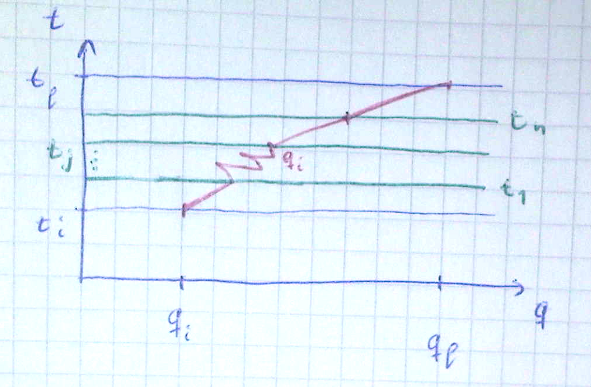
\includegraphics[width=0.75\textwidth]{kap05_01.png}


\(t_f-t_i = \tau(n+1)\)

\[ \langle q_ft_f|q_it_i\rangle =\int_{-\infty}^{\infty} dq_idq_2...dq_n\langle \overbrace{q_f}^{q_{n+1}}\overbrace{t_f}^{t_{n+1}}|q_nt_n\rangle \langle q_n t_n|q_{n-1}t_{n-1}\rangle...\langle q_{j+1}t_{j+1}|q_jt_j\rangle ...\langle q_1t_1|\underbrace{q_i}_{q_o}\underbrace{t_i}_{t_o}\rangle  \]

\[ \langle q_{j+1}t_{j+1}\rangle = \langle q_{j+1}|\underbrace{e^{-i\hbar t_{j+1}/\hbar}e^{i\hbar t_{j+1}/\hbar}}_{e^{-i\hbar \hat H (t_{j+1}-t_j)/\hbar}=e^{-i\hat H\tau/\hbar}}|q_j\rangle\approx 1-i\tau/\hbar \hat H + ... \]

\[=\underbrace{\delta(q_{j+1}-q_j)}_{\int_{-\infty}^{\infty}\frac{dp}{2\pi\hbar}e^{ip(q_{j+1}-q_j)/\hbar}}-\]

Annahme \(\hat H = \frac{\hat p^2}{2m}+V(\hat q)\)

\( \langle q_{j+1}|  \frac{\hat p^2}{2m} |q_j\rangle =\int dp'dp \underbrace{\langle q_{j+1}|p'\rangle}_{\frac{1}{\sqrt{2\pi\hbar}}e^{-ipq_{j+1}/\hbar}} \langle p'| \frac{\hat p^2}{2m} |p\rangle p \underbrace{\langle p|q_j\rangle}_{ \frac{1}{\sqrt{2\pi\hbar}}e^{-ipq/\hbar}} \)

\[  = \int \frac{dp}{2\pi \hbar}e^{i\frac{p}{\hbar}(q_{j+1}-q_j}\frac{p^2}{2m}\]


Normierung der \(|p\rangle \): \(\langle p|p'\rangle \delta (p-p')\); \(\langle p|q\rangle = \frac{1}{\sqrt{2\pi\hbar}}e^{-ipq/\hbar}\)


\[ \langle q_{j+1}|V(\hat q)| q_j\rangle  = V(q_j) \delta(q_{j+1}-q_j) = \int \frac{dp}{2\pi \hbar}e^{ip/\hbar(q_{j+1}-q_j)}V(q_j) \]

\[\langle q_{j+1}|e^{-i\hat H\tau/\hbar}|q_j\rangle = \int  \frac{dp}{2\pi \hbar} e^{ip(q_{j+1}-q_j)/\hbar}\overbrace{[1-i\frac{\tau}{\hbar}(\frac{p^2}{2m}+V(q_i))+...]}^{e^{-iH(p,q_i)\tau/\hbar}}\]

Für Propagator: 

\[\langle q_ft_f|q_it_i\rangle = \lim_{n \to \infty}\int...\int \prod_{j=1}^n(dq_j\frac{dp_j}{2\pi\hbar})\frac{dp_o}{2\pi\hbar}exp(\frac{i}{\hbar}\sum_{j=0}^n[p_j(q_{j+1}-q_j)-\tau H(p_j,q_j)])\]

\[= \int D_pD_q exp(\frac{i}{\hbar}\int_{t_i}^{t_f}dt(p(t)\dot q(t) - H(p(t),q(t)))\]

Sei \(\hat H = \frac{\hat p^2}{2m}+V(\hat q)\)

\[\langle q_f t_f|q_it_i\rangle = \lim_{n to \infty}\int...\int \prod_j dq_j \frac{dp_j}{2\pi \hbar} exp(i\sum_{j=0}^\infty(\underbrace{-\tau\frac{p^2_j}{2m}+\overbrace{p_j(q_{j+1}-q_j)/\hbar}^{2\sqrt{\frac{\tau}{2m\hbar}}p_j(q_{j+1}-q_j)/2\sqrt{\frac{\tau}{2m\hbar}}\frac{1}{\hbar}}}_{-(p_j\sqrt{\frac{\tau}{2m\hbar}}-(q_{j+1}-q_j)\sqrt{\frac{m}{2\tau\hbar}} )^2+\frac{m}{2\tau\hbar}(q_{j+1}-q_j)^2} - V(q_j)\frac{\tau}{\hbar})\]

\[= \lim_{n to \infty}\int \underbrace{\prod_{k=0}^n \frac{dp_k}{2\pi \hbar}e^{-\frac{i}{\hbar}\frac{\tau\hbar}{2m}p^2_k/\hbar^2}}_{\sqrt{\frac{2in\pi}{i\tau \hbar(2\pi)^2}}^{n+1}=\sqrt{\frac{m}{i2\pi\hbar\tau}}^{n+1}}\prod_{j=1}^n dq_j exp(\underbrace{\frac{i}{\hbar}\sum_{j=0}^n\tau(\frac{m}{2}(\frac{q_{j+1}-q_j}{\tau})^2-V(q_j))}_{\rightarrow \frac{i}{\hbar}\int_{t_i}^{t_f}dt(\frac{m}{2}(\dot q(t)^2-V(q))})\]


mit \(\int_{-\infty}^\infty dxe^{-\alpha x^2}=\sqrt{\frac{\pi}{\alpha}}\)


\[\langle q_ft_f|q_it_i\rangle = \lim_{n to \infty} \int \underbrace{(\frac{m}{2\pi i\tau \hbar})^{n+1}\prod_{j=1}^n dq_j}_{\mathcal D_q}e^{\frac{i}{\hbar}\int_{t_i}^{t_f}(\underbrace{\frac{m}{2}\dot q^2-V(q)}_{L(q,\dot q)})dt}\]

\[=\left.\int \mathcal D_q e^{\frac{i}{\hbar}\int_{t_i}^{t_f}dtL(q,\dot q)}\right|_{q(t_i)=q_i; q(t_f) = q_f}\]


Klassisches freies Teilchen

\[L = \frac{1}{2}mv^2\]

2 Pfade sind z.B. 
\begin{enumerate}
\item \(x_i(t) = vt\)  \(v=1\frac{cm}{sec}\)
\item \(x_2(t) = gt^2\) \(g = \frac{cm}{sec}\)
\end{enumerate}

Randbed. \(t_i = 0, x_i = 0, t_f = 1sec, x_f = 1cm\)

\begin{tabular}{ccc}
&\(m=1g\) & \(m=m_e\)\\
  \(x_1: S_1 = \frac{m}{2} v^2 t_f\)  &  \(4.7*10^26\hbar\) &   \(0.43\hbar\) \\
\(x_2: S_2 = \frac{2}{3} mg^2 t^3_f= \frac{4}{3}S_1\)  &&\\
\(S_2-S_1\) &  \( 1.6*10^26\hbar\)& \(0.14\hbar\)
\end{tabular}


In \(\int \mathcal D_q e^{\frac{i}{\hbar}S}\) extra \(\frac{1.6\cdot 10^{26}}{2\pi}\approx 10^{25}\) Oszillationen gegen \(S_1\)

Oszillation dämpfen Pfade mit \(S(q)>>S_{min}\)
Wichtig sind extremale Pfade mit \(\delta S = 0 \Leftrightarrow \) euler-Lagrange


\end{document}
